% generated by scripts/pkl_to_latex.py
% source PKL : vscan_v1_L6_Ne6_U10_t1_mode-uniform_nmin2_solver-gcg_full_restarts10_iter300_kmax5_tol1em09_V0to12_N25-ebabade1a2a1.pkl
% scan type  : vscan
% state      : gs
% quantity   : linear-entropy
% requires   : \usepackage{pgfplots} \pgfplotsset{compat=1.18}
% colours match the matplotlib PDF (tab10 cycle)
\definecolor{gmeC0}{HTML}{1F77B4}
\definecolor{gmeC1}{HTML}{FF7F0E}
\definecolor{gmeC2}{HTML}{2CA02C}
\definecolor{gmeC3}{HTML}{D62728}
\definecolor{gmeC4}{HTML}{9467BD}
\definecolor{gmeC5}{HTML}{8C564B}
\definecolor{gmeC6}{HTML}{E377C2}
\definecolor{gmeC7}{HTML}{17BECF}

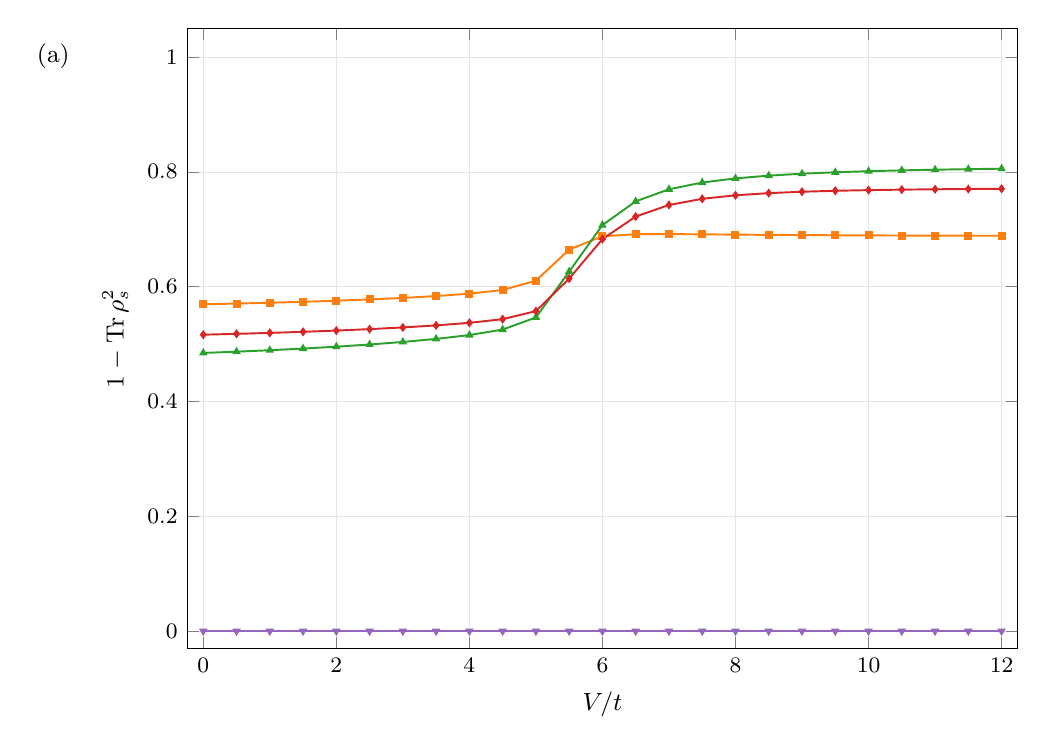
\begin{tikzpicture}
  \begin{axis}[
    width=\columnwidth,
    height=0.78\columnwidth,
    xlabel={$V/t$},
    ylabel={$1-\mathrm{Tr}\,\rho_s^2$},
    grid=both,
    grid style={line width=.1pt, draw=gray!20},
    tick label style={font=\footnotesize\rmfamily, /pgf/number format/fixed},
    label style={font=\small\rmfamily},
    scaled ticks=false,
    legend style={font=\scriptsize\rmfamily, draw=gray!40, at={(0.5,1.03)}, anchor=south, /tikz/every even column/.append style={column sep=6pt}},
    legend cell align={left},
    legend columns=2,
    ymin=-0.03,
    ymax=1.05,
    xmin=-0.24,
    xmax=12.24,
    after end axis/.append code={\node[anchor=east, font=\small\rmfamily] at (axis description cs:-0.13,0.954) {(a)};},
  ]
    \addplot[color=gmeC1, mark=square*, mark size=1.1pt, line width=0.7pt] coordinates {
        (0,0.569263) (0.5,0.570522) (1,0.571952) (1.5,0.57359)
        (2,0.57548) (2.5,0.57769) (3,0.580319) (3.5,0.583545)
        (4,0.587746) (4.5,0.594124) (5,0.610363) (5.5,0.664536)
        (6,0.687678) (6.5,0.691275) (7,0.691471) (7.5,0.691047)
        (8,0.690556) (8.5,0.690118) (9,0.689751) (9.5,0.689449)
        (10,0.689199) (10.5,0.688993) (11,0.68882) (11.5,0.688676)
        (12,0.688553)
    };
    \addplot[color=gmeC2, mark=triangle*, mark size=1.1pt, line width=0.7pt] coordinates {
        (0,0.484489) (0.5,0.486725) (1,0.489252) (1.5,0.492123)
        (2,0.49541) (2.5,0.499205) (3,0.503649) (3.5,0.508976)
        (4,0.515667) (4.5,0.525176) (5,0.546367) (5.5,0.626143)
        (6,0.70717) (6.5,0.74849) (7,0.769482) (7.5,0.781256)
        (8,0.7885) (8.5,0.793295) (9,0.796655) (9.5,0.799116)
        (10,0.800985) (10.5,0.802445) (11,0.803614) (11.5,0.804567)
        (12,0.805359)
    };
    \addplot[color=gmeC3, mark=diamond*, mark size=1.1pt, line width=0.7pt] coordinates {
        (0,0.516315) (0.5,0.517771) (1,0.519423) (1.5,0.521306)
        (2,0.52347) (2.5,0.525981) (3,0.528933) (3.5,0.532487)
        (4,0.536964) (4.5,0.543317) (5,0.557341) (5.5,0.614012)
        (6,0.682756) (6.5,0.722049) (7,0.742147) (7.5,0.752888)
        (8,0.759043) (8.5,0.76281) (9,0.765246) (9.5,0.766896)
        (10,0.768057) (10.5,0.7689) (11,0.76953) (11.5,0.770011)
        (12,0.770386)
    };
    \addplot[color=gmeC4, mark=triangle*, mark size=1.1pt, mark options={rotate=180}, line width=0.7pt] coordinates {
        (0,0) (0.5,0) (1,0) (1.5,-0)
        (2,0) (2.5,0) (3,-0) (3.5,0)
        (4,-0) (4.5,-0) (5,0) (5.5,-0)
        (6,0) (6.5,0) (7,-0) (7.5,-0)
        (8,0) (8.5,0) (9,-0) (9.5,0)
        (10,0) (10.5,0) (11,0) (11.5,0)
        (12,0)
    };
  \end{axis}
\end{tikzpicture}
